\documentclass[letterpaper,twocolumn,10pt]{article}
\usepackage{usenix-2020-09}
\usepackage{tikz}
\usepackage{amsmath}
\usepackage{hyperref}

%-------------------------------------------------------------------------------
\begin{document}
%-------------------------------------------------------------------------------

%don't want date printed
\date{}

\title{\Large \bf Towards CANLay: User-centered Overlay Design for In-Vehicle Data Dissemination In a Network Virtualized Testbed}

% %for single author (just remove % characters)
% \author{
% {\rm Jacob Jepson}\\
% Colorado State University
% \and
% {\rm Subhojeet Mukherjee}\\
% Colorado State University
% % copy the following lines to add more authors
% \and
% {\rm Jeremy Daily}\\
% Colorado State University
% } % end author

\maketitle

%-------------------------------------------------------------------------------
\begin{abstract}
%-------------------------------------------------------------------------------
Your abstract text goes here. Just a few facts. Whet our appetites.
Not more than 200 words, if possible, and preferably closer to 150.
\end{abstract}

\section{Introduction and Background}
%-------------------------------------------------------------------------------
In recent years security of the Controller Area Network (CAN) has been a much talked about topic of research. CAN is a broadcast media that enables reliable and low-latency communication between in-vehicle devices, also referred to as Electronic Control Units (ECU). This broadcast nature of CAN, along with the fact that it is inherently unauthenticated, makes it susceptible to network-wide cyber threats. 
Security researchers have shown \cite{checkoway_comprehensive_2011, mukherjee_practical_2016,burakova_truck_2016} that remote interfaces on modern vehicles can be used to intrude into internal CAN networks and inject messages to control and/or disrupt the operations of the vehicle. At the same time, the development of security solutions can be pursued to detect and/or prevent this scenario from occurring.
To evaluate the effectiveness of their methods, researchers have typically experimented on real-vehicles or homegrown testbed setups that mimic real vehicles. 
While most households in the United States have at least one passenger car\footnote{\url{https://www.statista.com/statistics/551403/number-of-vehicles-per-household-in-the-united}\\\url{-states/}}, this is not the same for medium and heavy-duty (MHD) vehicles. 
Moreover, creating homegrown testbeds is both logistically and economically challenging. To that end, the need for a publicly accessible testbench is imminent. This is where the concept of the Software Define Truck (SDT) \cite{mukherjee_towards_2021} is critical to the in-vehicle networking community. It aims to provide a distributed network virtualized platform on which in-vehicle security experiments can be performed. Although proposed primarily for the heavy-trucks, SDT can easily be adapted for lightweight passenger vehicles. SDT's information exchange goal is shown in figure \ref{fig:goal}. CAN frames and physical signals need to be exchanged between ECUs and vehicle simulators located in different subnetworks around the globe. CANLay is the networking backbone of the SDT and aims to provide the necessary infrastructure to enable this service.

\begin{figure}[t!]
    \centering
    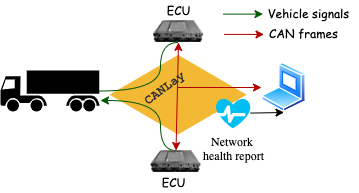
\includegraphics[width=\linewidth]{images/design_goal.drawio.png}
    \caption{Scope of CANLay}
    \label{fig:goal}
\end{figure}

Previous research \cite{tagarev_automotive_2021} has established two critical criteria for quality evaluation of automotive networking testbeds: fidelity and adaptability. Fidelity is the ability to emulate a real-world in-vehicle networking infrastructure. Adaptability is the ability to simulate different real-world in-vehicle networking infrastructures. As such, it may be difficult to optimize both at the same time. To make a system adaptable, the underlying components need to be virtualized so they can be reconfigured to suit user needs. Albeit, this hampers the fidelity of the system. While CANLay provides the means to configure experiment networks on-demand, it also provides a real-time health report for the underlying network. This allows the user to assess the fidelity of the overlay in terms of standard networking metrics like latency, rate of packet drop, etc.

Although, CAN is a relatively new communication technology and has a smaller application scope than TCP/IP, there has been some proposals to virtualize its operations. 
First, there has been the attempt to adapt the software-defined networking paradigm for CAN \cite{rotermund_requirements_2020,doering_retrofitting_nodate,grewe_bloomycan_2021}. This approach is largely hardware-based and is catered for in-vehicle networking on CAN physical channels, not over long-range overlays. For range relaying of CAN frames, there has been the CAN-to-ethernet direction of research \cite{johanson_relaying_2009,florian_polzlbauer_experience_2019}. The goal is not to enable ECU-to-ECU communication, rather transportation of data logged from one network to a remote endpoint. Configurability and network performance are usually not addressed. Neither is the CAN-to-ethernet paradigm designed to transport physical signals over long distances. 
X-in-the-loop (hardware, driver, vehicle etc.) simulation-based in-vehicle testbeds \cite{appel_safety_2020} have been proposed, but the signals from the simulators have been transported over physical connections, not over reconfigurable, long-range network overlays. 

In summary, CANLay provides the following features:
\begin{itemize}
    \item Transport of CAN frames and physical signals of the vehicle to a distributed network of electronic control units that can be located in different subnets
    \item Creation of these overlay CAN networks on demand
    \item Provision on runtime metrics to estimate the health of the network during the ongoing experiment.
\end{itemize}
In the rest of this paper we describe the design of CANLay (section \ref{sec:design}), provide a usability analysis (\ref{sec:usage}), and finish with conclusive remarks and future works.


% The distributed overlay nature of the project introduces a set of fidelity-related challenges when emulating the tightly integrated infrastructure within the vehicle. 
% Firstly, CAN provides a low-latency, strong reliability communication media that may be difficult to emulate over long-range communication channels. This requirement is even stronger for the physical signals that are usually transmitted over direct wiring in a real-world setting. 
% % A major requirement of this project is, therefore, to provide adequate assurance about the quality of communication in the overlay network. 
% Secondly, the broadcast nature of CAN may be difficult to realize in a distributed manner over the (typically) unicast internet protocols. Using unicast packets for multi/broadcast may require duplication in linear time. This is both space and time-intensive, especially if performed in a smaller scale local network that has limited bandwidth.
% The final challenge is to realize the complexity of interactions between the different components of the vehicle that normally operate in the same physical setting.
%TODO Dr. Daily, provide an example here




\section{Design and Current Development}\label{sec:design}
\begin{figure*}[t!]
    \centering
    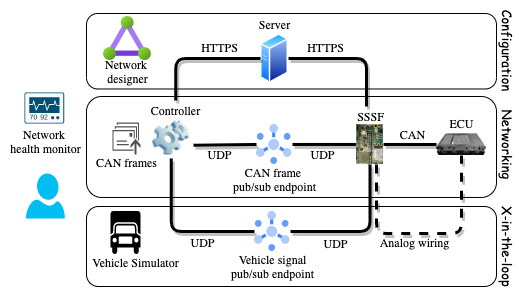
\includegraphics[width=\linewidth]{images/system_design.drawio.png}
    \caption{Proposed System}
    \label{fig:system}
\end{figure*}
Figure \ref{fig:system} shows the proposed system design of CANLay. The system serves three functions: offline configuration of the network overlay and CAN frame and vehicle signal exchange at runtime. A description of the components and their roles in the system is provided next. Following that, a description of the behavioral aspects of the system is provided. Together, these aspects combine to accomplish the functional objectives.

% ECUs in our system are required to interface with Smart Sensors Simulator (SSSF) devices. These devices act as gateways to the CANLay system. At startup they communicate with a central Server thereby registering themselves. This communication happens over HTTP(s). 

% \subsection{Current Status of Development}

\subsection{Component Descriptions}
\subsubsection{Smart Sensor Simulator and Forwarder (SSSF)}
The Smart Sensor Simulator and Forwarder acts as a gateway enabling the ECU to access and, more importantly, to be accessed by the CANLay system. In an active experiment, it acts as a forwarder between the Controller and the ECU through User datagram protocol (UDP) channels and CAN interfaces. SSSFs can forward two types of messages. 
The first type carries signals from the vehicle simulator. Eventually, these signals may have to be transmitted on the analog wiring that is shown using a dashed line figure \ref{fig:system}.  
The second type is CAN data carriers from the ECUs as well from other SSSFs in the current experiment. Through the SSSFs, multiple ECUs can actively communicate with each other to create a rich testing environment.

The SSSF is developed a built on a Teesny 3.6 .... a paragraph describing the SSS2's. Talk about SD cards. PLease include a blcok diagram etc.
CAN Forwarding 
%TODO Dr. Daily can help
The real time clock on the SSF is synchronized through the network time protocol (NTP).

\subsubsection{Controller}
The Controller is the user's interface to the CANLay system and enables vehicle simulators to communicate with the CANLay network. The Controller’s user interface is used to assist the user in building their virtual testbed. 
It does so by communicating with the central Server over hypertext transfer protocol secure (HTTPS). 
Once the experiment setup is completed the Controller transitions to acting as a gateway for a graphical vehicle simulator to communicate bi-directionally with the CANLay system. It forwards simulator outputs to the publish/subscribe (pub/sub) endpoint and listens for CAN messages from the same.

The Controller is a multi-threaded graphical application built using python. It is in charge of managing three subcomponents: the Vehicle Simulator, the Network Designer, and the Network Health Monitor. The Controller manages the execution of the Vehicle Simulator ensuring that it stays "in-step" with the flow of signals being produced. In addition, the Controller is in charge of updating the Network Designer's catalog of available devices as well as relaying the virtual network designs of user to the Server. The Controller efficiently manages the multiple streams of incoming and outgoing data through the use of Selectors. Selectors enable the Controller to know when a socket is available to read from or write to. Finally, once a session has begun, the Contoller manages the aggregation and presentation of network health reports. The Controller collects the current statistics from all devices in the session and displays the results in the form of heat matrices. These heat matrices will be discussed in-depth later on in the paper.

\subsubsection{Server}
The Server helps in setting up the publishers and subscribers for an experiment. Each device opens and must maintain a persistent transmission control protocol (TCP) connection with the Server while they participate in the CANLay system. Once the TCP connection is established the devices communicate with the Server through HTTP application programming interfaces (API). The Server can monitor the health of the devices and take actions if a device is malfunctioning or goes offline. This also allows the Server to keep track of free devices and free pub/sub endpoints, so it can validate new experiment requests and allocate the requested devices and endpoints without running into race conditions or double use issues that may arise if each Controller was in charge of allocating its own experiment. Finally, the Server keeps track of ongoing experiments and ensures the proper closure of a experiment in the event a device is experiencing issues.

The Server is a single-threaded session broker than multiplexes the handling of HTTP API calls through the use of Selectors. HTTP API calls were chosen because they clearly define the object to invoke and the manner in which to invoke it. The devices perform all necessary setup and teardown actions such as registering, deregistering, starting and stoping a session, by sending HTTP requests to different API endpoints. The Server responds to these requests using standard HTTP response messages and codes which can be easily interpreted by both the devices and users.

% \subsubsection{Vehicle Simulator}
% In theory, the Vehicle Simulator can be any software that provides the user with the ability to control a vehicle in a digital world. To be compatible with CANLay, the Vehicle Simulator must expose its operating signals in some manner. For the purpose of this paper, we chose the CARLA graphical vehicle simulator \cite{Dosovitskiy17}. 

% Although the Carla project mainly focuses on autonomous driving research it exposes its in-game signals through an easy-to-use python api and pays close attention to the scientific details represented in its simulator. While this is not required, the more realistic and accurate the signals are, the easier it will be to transform them into CAN messages. Furthermore, CARLA is highly configurarble, robust and has been used for purposes similar to ours.

% \subsubsection{User Interface to CAN}
% We forward the recieved CAN frame on a virtual CAN (VCAN) interface that is provided by the user at startup. A user can access these frames via socketCAN \footnote{\url{https://www.kernel.org/doc/html/latest/networking/can.html}} and assosiated tools.

\subsubsection{Publish/Subscribe Endpoints}
UDP is used to connect the publishers and subscribers in the CANLay system. 
% A pub/sub endpoint in the CANLay network is a pub/sub address and port pair. Although the CAN frame and Vehicle signal pub/sub endpoints are shown separately in the above diagram for clarity, they are physically a single endpoint in the network. 
The pub/sub model was chosen because it can easily emulate the broadcast nature CAN \cite{kaiser_implementing_1999} in that an ECU is subscribed to all other ECUs on the same CAN bus and all other ECUs on that CAN bus are subscribed to that ECU. 

To find a suitable pub/sub mechanism that closely resembles a CAN network, we used a few criteria. The first is that the transport mechanism must support some form of message broadcasting that enables a sender to send one message that can be received by many receivers without significant duplication and delay-related overheads \cite{kaiser_implementing_1999}. The next requirement is that the transport mechanism must enable the devices to receive messages from one or more devices while having to maintain only one connection.
% In addition the transport mechanism must not have any implicit congestion control or flow control since none is found in CAN networks. Finally, it's preferable if the communication mechanism transported data as individual messages rather than streams of data.

At this time we have chosen UDP multicasting as a suitable pub/sub mechanism as it does not require a message broker with high-performance requirements. We realize that multicasting outside a local network may lead to increased cost for the implementers, but the current goal was to test its usability and make future decisions based on the observed performance. At this time, we are also exploring other potential pub/sub implementations such as MQTT.


\subsubsection{Front-End Components}

\begin{figure*}[t!]
    \centering
    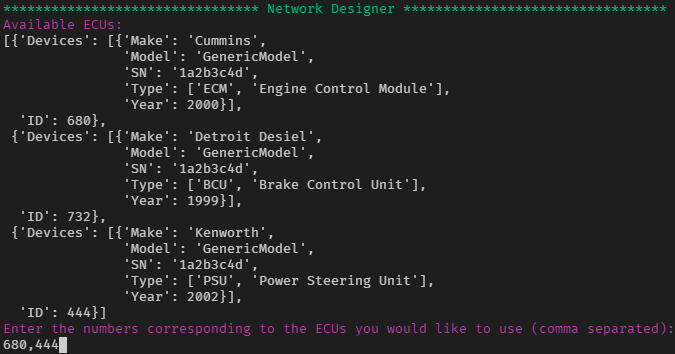
\includegraphics[width=\linewidth]{images/network_designer.png}
    \caption[]{Network Designer displaying available ECUs\protect\footnotemark}
    \label{fig:network_designer}
\end{figure*}

The Network Designer consists of a catalog of available devices and the ability to select the requested devices. Upon start up the Controller contacts the Server and requests the latest set of avaialble devices. The Controller then presents these options to the user and allows them to select the request devices from the catalog of available ECUs.

\footnotetext{Currently the network designer is controlled through the command line but in the future a GUI will be added that performs the same function.}

\begin{figure}[t!]
    \centering
    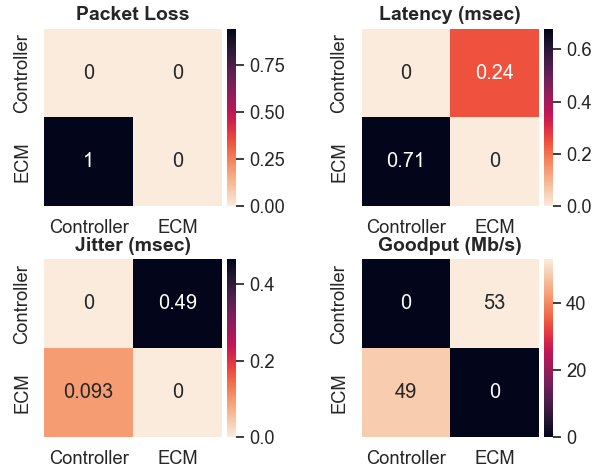
\includegraphics[width=\linewidth]{images/network_matrix.png}
    \caption[]{Network Matrices showing packet loss, latency, jitter, and goodput.}
    \label{fig:network_matrix}
\end{figure}

The Network Health Monitor shows real time network statistics that describe the current state of the network. These statistics are presented using heat matrices. Each cell in the matric represents a directed edge of the network. The color of the cells depends on their values. For packet loss, latency, and jitter the lower the number the better and the lighter the color will be. For goodput the higher the number the better and the lighter the color will be. The contrast between the light and dark colors allows the user to quickly spot parts of the network that are underperforming.


% A large drawback of connecting devices over a shared/multipurpose network is the increase of networking delays. When a user creates a virtual test bed using CARLay they are logically forming a virtual network for that experiment, but physically each device is still connected to the same network as before. As a result, communication between devices in a virtual test bed could suffer from network delays that are out of the user’s control. 
% The Network Health Monitor provides the user with useful information about the current status of the network so they can ensure that the current network conditions are not affecting their results. 
% The network information is gathered from the perspective of all devices in a experiment rather than collecting it from just the perspective of the Controller. This provides a more full view of the current state of the network.

\begin{figure*}[t!]
    \centering
    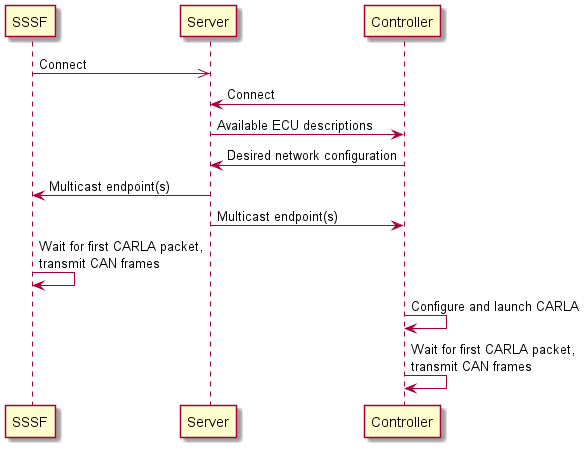
\includegraphics[width=\linewidth]{out/images/connection_setup/connection_setup.png}
    \caption{Setup Activity}
    \label{fig:setup_activity}
\end{figure*}

\subsection{Behavior Descriptions}
\subsubsection{Setup (ref. figure \ref{fig:setup_activity})}
While the Server is up and running SSSFs connect to it. SSSFs perform a setup(the) procedure by reading their inbuilt SD card. The type, year, make, model and a serial number of the connected ECUs are required to be included in a predefined file stored on the SD card. Next, the SSSF gathers its MAC address and list of attached devices into a JSON and sends it to the Server via a POST to the HTTP API endpoint /\textit{SSSF}/\textit{Register}. 
% The Server will parse and validate the registration. If the registration is satisfactory, it will reply with a code 202 indicating to the SSSF that it has successfully registered with the Server. 
% If the registration data contains invalid data such as a  attached device, or invalid JSON the Server will respond with the appropriate error code and drop the connection.
If the registration fails, the Server responds with a HTTP 4XX error code indicating why the registration failed. Otherwise, the Server responds with a HTTP 202 code indicating the SSSF was accepted. Once successfully registered, the SSSF waits for further instructions from the Server on its TCP/HTTPS port. 

The Controller begins by registering with the Server in a similar manner to the SSSF except that the Controller has no attached devices so it only sends its MAC address to the Server.
% The Server will once again pars/e and validate the registration and respond with the appropriate code. If the Controller successfully registered then it proceeds to make a “GET” to the HTTP API endpoint “\\SSSF”. 
Once successfully registered, the controller requests a list of the available{\footnote{If a SSSF device is currently being used in another experiment it is not considered available.}} SSSF devices. After receiving the list of available devices, it presents the available ECUs to the user via the Network Designer described above. Notice that while the Server deals with the SSSF devices a user will typically only be interested in the ECUs that the SSSF is acting as a gateway for. After the user finalizes their selection, the Controller sends the selected devices to the Server via a HTTP POST and waits for the Server's reply.

The Server receives the list of requested devices and performs three checks. First, it checks that the request is coming from a registered Controller. Controllers are the only devices allowed to start sessions. Next, the Server double checks that the devices are still available. If any of the devices are no longer available or become unavailable during the setup process, the Server responds to the Controller with the error code 409 indicating there's a conflict in the selection. If all of the devices are still available, the Server then selects an available pub/sub endpoint for the experiment and assigns an index to each device. The index aids in the the collection of network statistics which will be explained later on. At this time the Server sends the connection data to the Controller and selected SSSFs. Connection data contains the unique ID and index of the device, a multicast IP address and port acting as the pub/sub endpoint, and a list containing the IDs and attached devices of other nodes in the experiment.

Once endpoints receive the connection data they resync with NTP, allocate space for the required data structures, and begin listening for and forwarding messages to and from the pub/sub endpoint. At this point the experiment setup is completed.

\subsection{Network Setup}

\subsection{Data Transport}
\begin{figure}[t!]
    \centering
    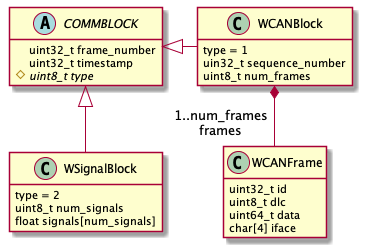
\includegraphics[width=\linewidth]{out/images/data_structures/data_structures.png}
    \caption{Transport Data Structures}
    \label{fig:ds}
\end{figure}
\subsubsection{Sensor Communication}
% The CANLay framework lays the foundation for X-in-the-loop simulation and testing.
% Before we can transform graphical vehicle simulator signals into CAN messages, there must first be a way for the in-game signals to reach the SSSF simulator and the CANLay framework achieves just that. 

Once an active session has been established the Controller begins forwarding sensor signals to the pub/sub endpoint. Before sending out the sensor signals the Controller wraps them in a WSensorBlock and then a COMMBlock. There are several additional pieces of information the COMMBlock requires, but we'll focus on type and frame number for now. The type indicates the subclass that the COMMBlock is carrying. In this case the type will be 2, indicating that it is carrying a WSensorBlock. The frame number is added to the COMMBlock and is incremented by 1 everytime the Controller forwards a Sensor message to the CANLay network. When SSSFs send out CAN messages they’ll set their outgoing COMMBlock's frame number to the last received frame number from the Controller. When the Controller receives CAN messages, it'll read the frame number field and know the last Sensor message that the SSSF received. This creates an acknowledgment feedback loop enabling the Controller to tell which devices have received a frame and when a frame has been lost. This acknowledge feedback loop is possible because CAN messages are sent at a higher rate than the sensor message are. This enables an acknowledge mechanism that does not require any additional messages.

Before starting the session the user Controller lets the user select the maximum number of retransmissions which is then used to calculate the timeout value of a Sensor frame. The timeout value is calculated as follows: $1/(simulator\_frame\_rate * max\_retransmitions)$. When the Controller detects that the last frame has timed out, it first checks if it has reached its maximum number of retransmissions. If not it'll resend the Sensor message, increment the number of retransmissions its performed, and reset the time out timer. It’ll repeat this process until it either receives a CAN message with a frame number equal to the Controller's current frame number or it reaches the maximum number of retransmissions. In the later case, the frame is considered lost and the Controller moves on.

As mentioned before, when a SSSF receives a Sensor frame it first sets its last seen frame number equal to the message's frame number. Next the SSSF applies any necessary transformations to the Sensor frame before forwarding it on to its device's CAN network(s). For the purposes of this paper the transformations served mainly as a proof of concept and were kept simple, often sending just the raw sensor value in with the closest matching PGN CAN frame.

\subsubsection{CAN Communication (ref. figure \ref{fig:can_x})}
\begin{figure*}[t!]
    \centering
    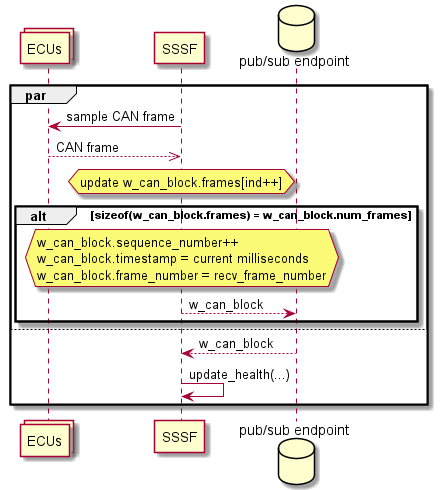
\includegraphics[scale=0.8]{out/images/can_exchange/can_exchange.png}
    \caption{CAN Communication Activity}
    \label{fig:can_x}
\end{figure*}
% In order to create the simulated CAN network of ECUs, the devices must be able to communicate with each other with minimum per
% as if they were talking via a CAN bus. 
% Most ECUs do not come with built in ethernet ports and the ability to broadcast CAN frames via Ethernet. So in order to connect an ECU to Ethernet we need a device that can interface with a CAN network and interface with an Ethernet Network. This is why 
% the Smart Sensor Simulator and Forwarder is necessary. It acts as a programmable gateway that can transfer messages between the CAN network and the Ethernet Network.

When the SSSF is in an active experiment it attempts to read a message from the CAN network. Upon doing so, it creates the COMMBlock data structure (ref. figure \ref{fig:ds}) that will be written to the CANLay network. 
% In the current scenario we set \texttt{num\_frames} to 1. Therefore, a COMMBlock data structure is transmitted after the receipt of every message.
Before the COMMBlock is written to the network addition information is added. There are several additional pieces of information required, but we'll focus on three right now. Namely, type, sequence number, and needs\_response. The type indicates the subclass that the COMMBlock is carrying. In this case the type will be 1, indicating that it is carrying a WCANBlock. The sequence number is added to the WCANBlock and is incremented every time a CAN message is sent from the device. Since the message rates of Sensor and CAN messages are asymmetrical the acknowledgement mechanism described in the previous section only works in one direction. However the sequence number included in the WCANBlock is still used for acknowledgements and to detect pack loss. The packet loss mechanism is described in detail in the Network Health Monitoring section. The acknowledgement mechanism for CAN messages works differently compared to the acknowledgement mechanism described before. Whereas every Sensor message is implicitly acknowledged, CAN messages are explicitly acknowledged when \textit{needs\_response} is set to true. The field \textit{needs\_response} is set to true if its CAN frame’s PGN matches a list received from the user during setup.

After the SSSF is done checking for CAN messages from the CAN network, it moves on to check for messages from the pub/sub network. Again, CAN messages sent to the pub/sub endpoint are considered type 1 messages. So if an SSSF device receives a type 1 message it first checks if the message requires a response. If so, it replies to the pub/sub endpoint with a type 5 message with the frame number equal to the sequence number of the message it just received. Finally, the SSSF updates its network statistics and then it extracts the WCANFrame and writes it onto its available CAN networks.
\begin{verbatim}
if (msg.type == 1)
{
    if (msg.needsResponse)
    {
        writeToMcastEndpoint(5. msg.seqNum);
    }
    networkHealth->update(msg);
    if (can0BaudRate) can0.write(msg.canFrame);
    if (can1BaudRate) can1.write(msg.canFrame);
}
\end{verbatim}

\subsubsection{Network health monitoring}\label{sec:nethealth}
\begin{figure}[t!]
    \centering
    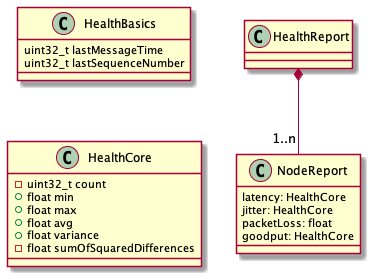
\includegraphics[width=\linewidth]{out/images/network_health/network_health.png}
    \caption{Network Health Data Structures}
    \label{fig:network_health_ds}
\end{figure}
Monitoring the health of the network is key to ensuring that bad delays or large amounts of packet loss are not affecting your test results. In order to enable the devices to collect network statistics during an active experiment, each message is loaded with additional information. The first piece of additional information is a frame or sequence number. When other devices spot gaps in these numbers larger than 1 they know that a message has been lost.
% The Controller increments the frame number everytime it sends out new signals. When the SSSFs receive a message with a frame number higher than the previous frame number they saw, they set their frame number to the new frame number. Whenever SSSF devices send a message they append the latest frame number to the top of it. When a Controller receives a CAN message it checks the frame number included in the message. This tell the Controller the last frame the device had received when it sent the CAN message. This system enables acknowledgement of messages without having to send any additional messages. In addition if an SSSF spots a gap in the frame numbers that is larger than 1, then it knows that a frame has been lost.

% The type 1 COMMBlock messages (messages containing CAN frames) include a sequence number in addition to the frame number discussed earlier. Whenever an SSSF device sends out a CAN message, it adds a sequence number and increments it by 1. Signals from the Controller are sent at the frame rate of the game. This means that with a frame rate of 60fps the Controller is sending messages about 3-4x slower than the message rate seen in on a 250,000 baud ECU operating at nominal bus load. As such we cannot expect the acknowledgement mechanism used for the Controller messages to work for the CAN messages. However other devices can still use the sequence numbers to detect dropped CAN messages by looking for gaps larger than 1.

The next important metric included in the COMMBlock messages is a timestamp. Timestamp is included to allow devices to calculate the latency along the network edge from the sending device to the receiving device.
% Of course this could be done by performing network tests during an active experiment but unless the latency is guaranteed to always be low, this testing could interrupt the normal flow of the other messages being sent in the experiment.
The timestamp is included with each message that is sent so that network health metrics can be calculated without interrupting the testing. The latency is calculated by subtracting the time at which the message was sent from the time at which the message was received. To ensure accuracy every device on the CANLay network implements NTP to synchronize their clocks.
% The downside to this method is that it requires all of the device's clocks to be synchronized as close as possible. With the current basic implementation of the NTP protocol, the devices on average stay within a millisecond or two of each other when they are all referencing an NTP Server on the same network. Unfortunately when the devices use different NTP Servers that are much farther away the devices tend to stray between 5-15 milliseconds from each other. This creates issues when trying to measure the latency of devices that are very close to each other. It's important to note that more advanced implementations of NTP may be able to shrink these numbers.

These indicators enable each device to calculate four network statistics for every other device on the network. Currently these statistics include packet loss, latency, jitter, and goodput. Packet loss is the number of packets determined to be lost along a network edge. Latency is the time it takes a message to travel from the sender to the receiver. Jitter is the variance in latency. There are many different types of network jitter but we use the simplest form which is often called packet jitter or constant jitter. Packet jitter is defined as “the variation in latency as measured in the variability over time of the end-to-end delay across a network”
% what form do we cite in for this publisher?
(cite https://networkencyclopedia.com/jitter/). Finally, goodput is the measurement of application level throughput. In our case it is calculated as Megabits per second.

To display these captured statistics to the user the Controller needs to first aggregate the Health reports from every device. The Controller does so every second by sending out a type 3 message which requests the health report from each device. After each device has replied with their health report they reset their statistics, keeping only the last message timestamp and the last seen sequence number. This creates a measurement period of 1 second. As the Controller receives the health reports, it updates the network statistic data structure and displays the new results to the user.
\begin{verbatim}
update(i, packetSize, timestamp, seqNum)
{
    now = timeClient->getEpochTimeMS();
    delay = now - timestamp;
    ellapsedSeconds = (
        now - HealthBasics[i].lastMessageTime);
    ellapsedSeconds /= 1000.0;

    calculate(Report[i].latency, abs(delay));
    calculate(
        Report[i].jitter,
        Report[i].latency.variance
        );

    // If no packet loss then sequence number
    // is equal to last sequence number + 1
    pcktsLost = seqNum - (
        Basics[i].lastseqNum + 1);

    // If pcktsLost is negative then this
    // indicates duplicate or out of 
    // order frame.
    Report[i].pcktLoss += (
        pcktsLost > 0) ? pcktsLost : 0;

    calculate(
        Report[i].goodput,
        (packetSize * 8) / ellapsedSeconds
        );
    
    HealthBasics[i].lastMessageTime = now;
    HealthBasics[i].lastseqNum = seqNum;
}

calculate(HealthCore &edge, n)
{// From: https://en.wikipedia.org/wiki/
Algorithms_for_calculating_variance#
Welford's_online_algorithm
    edge.min = min(edge.min, n);
    edge.max = max(edge.max, n);
    edge.count++;
    delta = n - edge.mean;
    edge.mean += delta / edge.count;
    delta2 = n - edge.mean;
    edge.sumOfSqrdDiffs += delta * delta2;
    edge.variance = 
        edge.sumOfSqrdDiffs / edge.count;
}
\end{verbatim}


\section{Current Implementation}\label{sec:usage}
\begin{figure*}[t!]
    \centering
    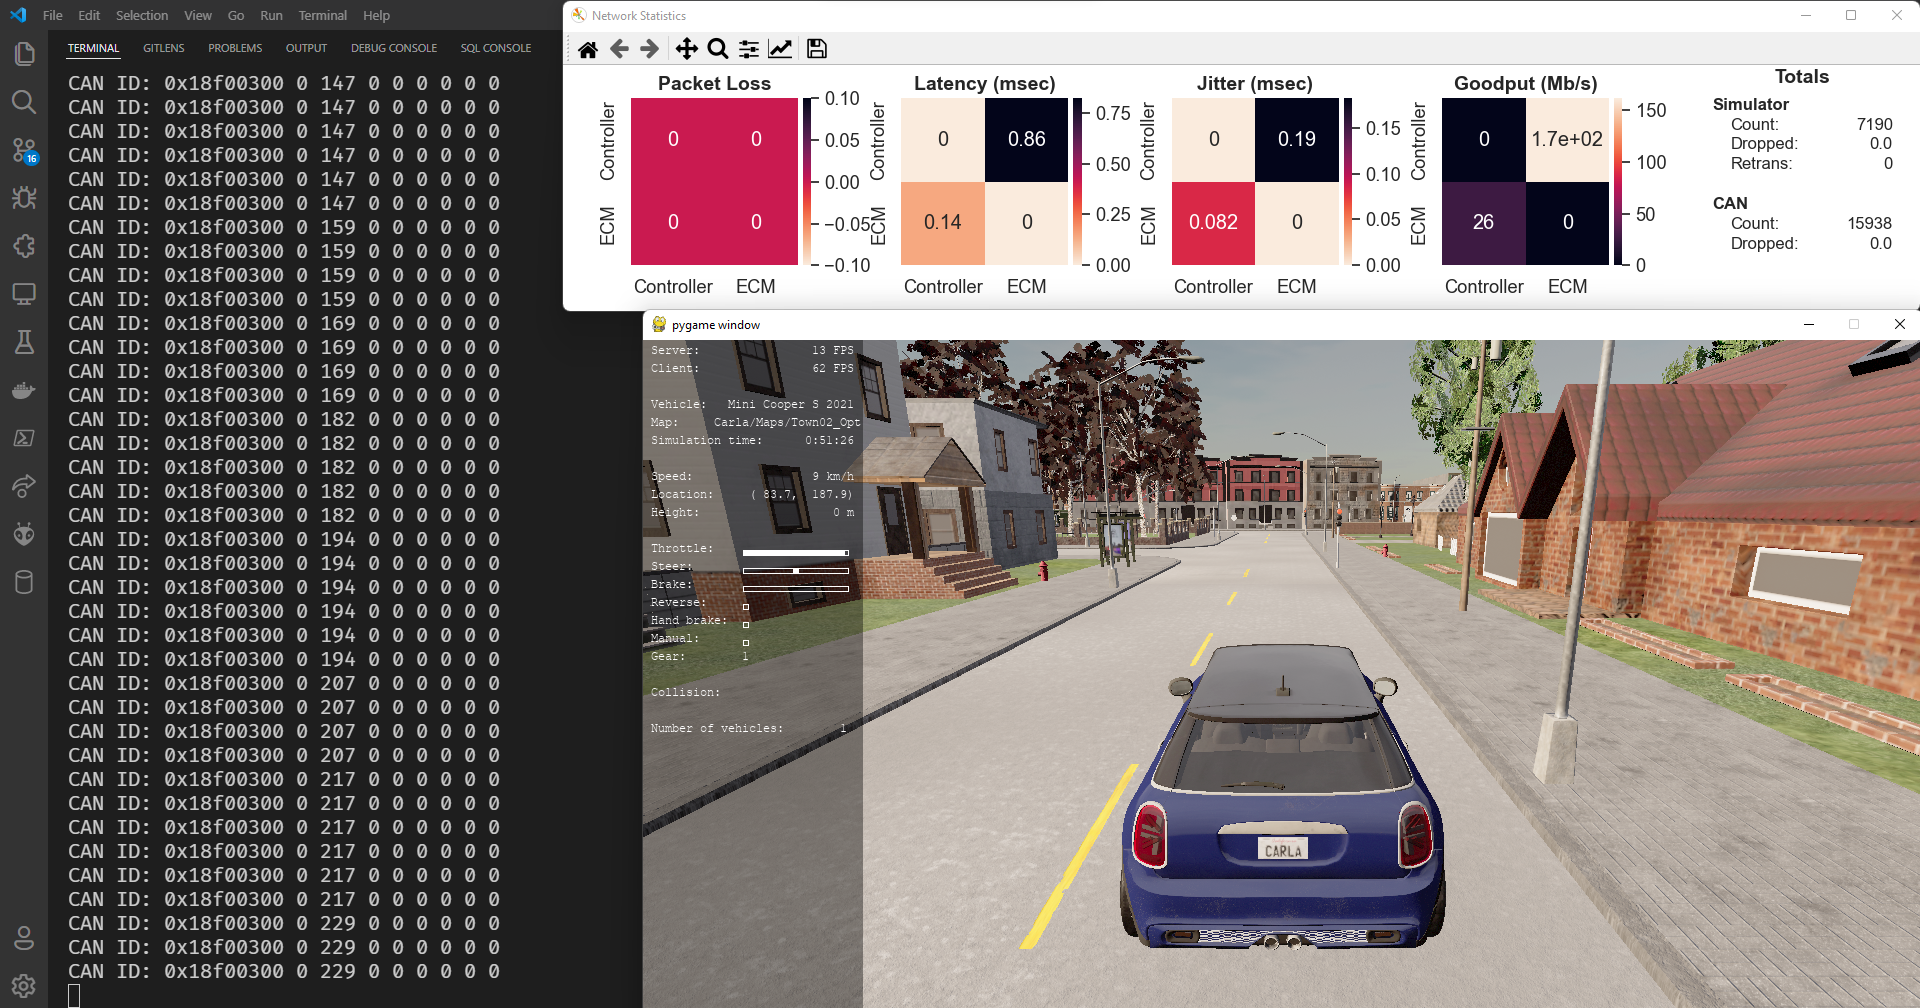
\includegraphics[width=\linewidth]{images/usability.png}
    \caption{CANLay at work in the Software Defined Truck}
    \label{fig:usabiity}
\end{figure*}
Figure \ref{fig:usabiity} shows CANLay at work. The windows in the figure display CAN frames on left, the vehicle simulator on the bottom right and CANLay's network health monitoring on the top right. Each of these components were already introduced in figure \ref{fig:system}. For the current purpose we have been using the CARLA graphical vehicle simulator \cite{Dosovitskiy17}. 
Although the Carla project mainly focuses on autonomous driving research it exposes its in-game signals through an easy-to-use python API and pays close attention to the scientific details represented in its simulator. While this is not required, the more realistic and accurate the signals are, the easier it will be to transform them into CAN messages. In this case, a specific CAN frame is printed as they are broadcasted on the overlay for this particular experiment. The ID of this frame is defined by the SAE-J1939 standards \cite{society_of_automotive_engineers_sae_nodate} and identifies engine parameters transmitted by an engine control module (ECM). The data bytes carried in the CAN frame are shown next. Of these, the third byte is shown to be changing. This particular byte carries the percentage throttle demanded by the driver. The value is also non-zero on the simulator frontend provided by the CARLA simulator.

On the top right is the network health monitoring window. It shows four matrices showing
four different metrics to estimate network health: packet loss, latency, jitter, and goodput. The significance of each of these metrics and their calculation methods were already described in the previous section. In this case, the experiment is performed over a gigabit local area network with a layer 3 switch in between an SSSF and a Controller. The figure shows no packets were lost while the latency in the last cycle of health report collection was about 4 milliseconds between the endpoints. Although CANLay does not explicitly perform any latency reducing functions, the general latency of 4 milliseconds is considered to be sustainable for seamless CARLA emulation at standard frame rates. In this particular example, the CARLA emulation frame rate was chosen to be 60 frames per second. The jitter is also fairly low in comparison to the latency. The goodput, i.e. the application data rate is understandably higher for the Controller as it sends WSignalBlock frames that are slightly larger than the WCANBlock frames. 

\section{Conclusion and Future Work}
In this paper, we described the concepts behind the design of CANLay, the networking backbone for the Software Defined Truck. SDT is a virtualization based experimentation framework for CAN-based security experiments and CANLay is the carrier of physical control and CAN data over long distance networks. Essentially CANLay enables network virtualization for SDT. CAN is a reliable and low-latency network. CANLay does not explicitly ensure reliability and low latency, but provides a health monitoring service that provides real-time measures of network parameters to the user. This allows the user to make critical decisions about the state of the experiment they are in.

We believe more than one additional works can still be done on CANLay. 
Need response
Dynamic buffer adjustment
 
%-------------------------------------------------------------------------------
\bibliographystyle{plain}
\bibliography{bib}

%%%%%%%%%%%%%%%%%%%%%%%%%%%%%%%%%%%%%%%%%%%%%%%%%%%%%%%%%%%%%%%%%%%%%%%%%%%%%%%%
\end{document}
%%%%%%%%%%%%%%%%%%%%%%%%%%%%%%%%%%%%%%%%%%%%%%%%%%%%%%%%%%%%%%%%%%%%%%%%
